\documentclass[final]{tikzposter}
\usepackage{geometry} % Load without options
%\geometry{paperwidth=17in, paperheight=11in, margin=0.5in} % Set dimensions afterward
%\geometry{paperwidth=32.5in, paperheight=33in} % Set dimensions afterward
\usepackage{kotex}
\usepackage{xcolor}
\usepackage{hyperref}
\usepackage{commath}

\usepackage{adjustbox}

\usepackage[T1]{fontenc}
\usepackage{lmodern}
\usepackage{amsmath,amssymb}
\usepackage{graphicx}
\usepackage{fontawesome5} % For decorative icons

% Define custom colors
\definecolor{csesky}{HTML}{49b7ad} % csesky
\definecolor{cseblue}{HTML}{003a8a} % cseblue

\usetheme{Wave}
\usecolorstyle[colorPalette=Default]{}

% Override default colors with custom ones
\colorlet{titlebgcolor}{csesky}         % Title background color
\colorlet{titlefgcolor}{white}          % Title text color
\colorlet{blocktitlebgcolor}{csesky}      % Block title background color
\colorlet{blocktitlefgcolor}{cseblue}     % Block title text color

\definecolor{titlecolor}{HTML}{b9515c}
%\title{\fontsize{120}{5}\bfseries \textcolor{titlecolor}{Mathematics Seminar / 전공수학 세미나}}
%\title{
\includegraphics[scale=4.15]{title.pdf}}
\title{\centering
\includegraphics[width=.8\textwidth]{title.pdf}}
\author{\textbf{Instructor:}\ 
%	
\includegraphics[scale=4]{jyh.pdf}
	\textcolor{yellow}{\bfseries Ji, Yong-hyeon / 지용현}
}
\institute{Department of Cyber Security / 사이버보안학과\\ Kookmin University / 국민대학교\\ [2cm] Spring 2025}
\titlegraphic{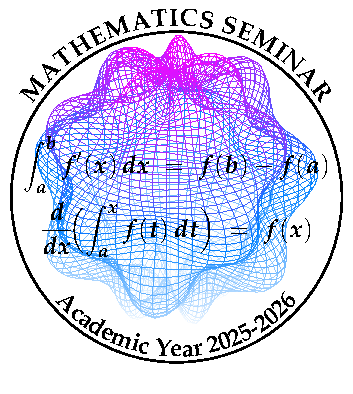
\includegraphics[scale=4]{poster-cover.pdf}} % Replace with your logo/image

\begin{document}
	\maketitle
	
	\begin{columns}
		\column{0.5}
		\block{\Huge Course Overview / 과정 개요}{
%			\vspace{10pt}
			\Large
			\textbf{\color{teal}``전공수학 세미나''} 스터디는 학과, 학년 관계 없이 누구나 참여 가능한 학부
			및 대학원 수준의 전공수학을 포괄적으로 다룹니다. \\
			{\color{gray}(다만, 교양수학이 아닌 `전공'수학을 하기 때문에 난이도는 있습니다.)}\\
			\begin{itemize}
				\item \bfseries 집합론 (Set Theory);\hfill $\color{magenta}\forall X,\ |X|<|\mathcal{P}(X)|$
				\item 해석학 (Analysis); \\$\color{magenta}
				\lim\limits_{x\to c}f(x)=f(c)\iff\forall\varepsilon>0,\ \exists\delta>0,\ |x-c|<\delta\Rightarrow|f(x)-f(c)|<\varepsilon$
				\item 일반위상수학 (General Topology);\\ $\color{magenta}
				\text{\normalfont $X$ is compact}\iff\forall\mathcal{U}, (X\subset\cup\hspace{1.5mm} \mathcal{U}\Rightarrow \exists\mathcal{U}_0\ \text{\normalfont s.t.}\ |\mathcal{U}_0|<\infty\ \text{\normalfont and}\ X\subset \cup\hspace{1.5mm}\mathcal{U}_0)
				$
				\item 선형대수학 (Linear Algebra);\hfill $\color{magenta}\dim V=\dim(\ker T)+\dim (\text{\normalfont Im}\ T)$
				\item 추상대수학 (Abstract Algebra);\hfill $\color{magenta}G/\ker f\simeq \text{\normalfont Im}\ f$
%				\item 측도론 (Measure Theory);\hfill $\color{magenta}m^*(E)=\inf\set{\Sigma_{n\geq 1}\ell (I_n)\mid E\subset \cup_{n\geq 1} I_n}$
			\end{itemize}\ \\ 와 같은 다양한 전공수학 과목들을 논리적으로 폭넓게 서로 유기적으로 학습함으로써, 보다 높은 수준의 수학적 사고와 연구 역량을 키우는 것을 목표로 합니다. 다양한 배경을 가진 학생들이 어렵기만 느껴지는 {\bfseries\color{blue}\underline{수학을 함께 즐기고 공감하며 배울 수 있는 장}}을 제공하고자 합니다.
		}
		
		\block{\Huge Course Objectives / 과정 목표}{\Large
			\begin{itemize}
				\item {\bfseries\underline{고급 수학적 사고와 수학적 증명 및 논증을 훈련}.}
				\item {\bfseries\underline{현대 수학 이론 전반에 걸친 심도 있는 유기적 이해 증진}.}
%				\item {\bfseries\underline{다양하고 복잡한 여러 수학 분야의 개념을 통합}.}
			\end{itemize}
		{\color{red}* 커리큘럼은 ``\underline{\bfseries (집합론)\hspace{-.25cm} $\to$\hspace{-.25cm} (해석학 \hspace{-.3cm}+\hspace{-.3cm} 기초 위상)\hspace{-.25cm} $\to$\hspace{-.25cm} (선형대수학 \hspace{-.3cm}+\hspace{-.3cm} 군론)}''으로 구성되어 있으며 각 과목을 자세하고 아주 깊이 이해하기 보다는 여러 \underline{\bfseries 전공수학 과목 간의 큰 그림을 이해}하는 데 목표로 하고 있습니다.}
		}
		\block{\Huge Who Should Join / 참여대상}{\Large
			\begin{itemize}
				\item \bfseries\underline{함께 이야기를 나누고, 토론하고, 공감하며 수학을 배우고 싶은 분}.
%				\item \bfseries\underline{전공수학을 제대로 공부해 보고 싶은 분}.
				\item \bfseries\underline{전공수학 수업을 들어봤는데 막상 잘 모르겠고 남는 것이 없는 분}.
				\item \bfseries\underline{전공수학 과목들이 어떻게 유기적으로 연결되어 있는지 알고 싶은 분}.
			\end{itemize}
%			서로 다른 배경을 가진 학생들이 수학 이야기를 나누고, 토론하고, 공유함으로써 함께 배우는
%			공동체를 만들어 가고자 합니다. 학년이나 배경에 상관없이 수학에 열정을 가진 모든 분들을 환영합니다.
		}
		\column{0.5}
		\block{\Huge Course Materials / 교재}{\Large
			전 과목에 대해 고퀄리티 자체 제작 강의노트를 제공합니다.
			\begin{center}
				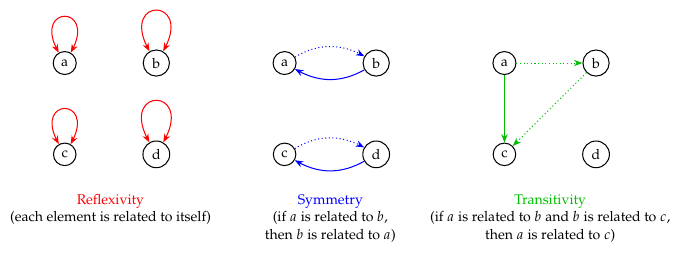
\includegraphics[width=.46\textwidth]{lecture-note-1}
				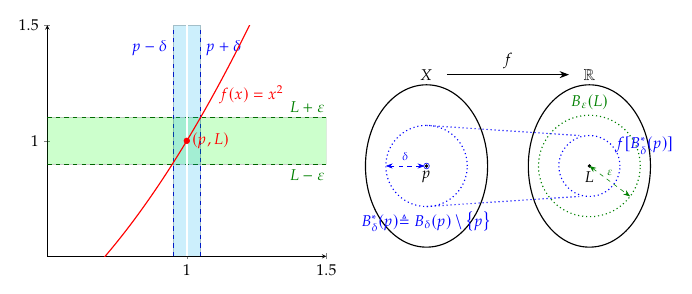
\includegraphics[width=.46\textwidth]{lecture-note-4}
%				\caption{Set Theory (Equivalence Relation)}
			\end{center}
			
%			\begin{figure}[h!]\centering
%				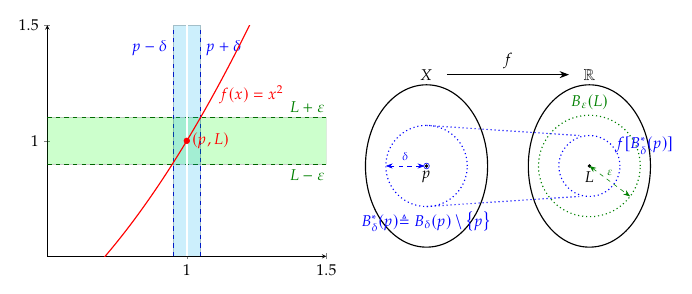
\includegraphics[scale=.4]{lecture-note-4}
%				\caption{Advanced Calculus ($\varepsilon-\delta$ method)}
%			\end{figure}
			
%			\begin{figure}[h!]\centering
%				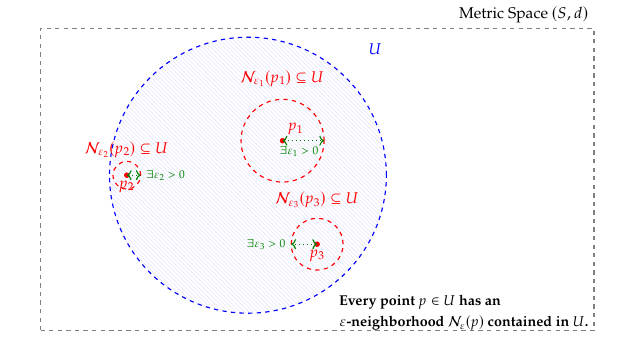
\includegraphics[scale=.4]{lecture-note-3}
%				\caption{Topology (Neighborhood)}
%			\end{figure}
		}
		
		\block{\Huge Period / 모집기간}{\Large
			\textbf{\color{blue}\underline{2025. 03. 04 - 03. 14}} (오리엔테이션은 3월 2주차 (3.10 - 14)에 진행)
			\\ \\
			\small\color{red} * 모집기간과 별도로 오리인테이션을 진행하며, 모집 기간 이후에 참여를 원하시면 언제든 이메일로 연락바랍니다.
		}

		\block{\Huge Apply / 지원방법}{\Large
			기타 문의사항은 아래 이메일, 참여신청은 구글폼 링크에서 가능합니다.
%			\bigskip
			
			\begin{center}\large
				\faEnvelope\ \texttt{hacker3740@kookmin.ac.kr} \quad\quad
				\faGlobe\ \texttt{\color{red}\url{https://forms.gle/RzS8tGzXstXZ1XNW9}}
			\end{center}
		}
	\end{columns}
	
\end{document}
